% Probability mass functions tell us how probable each sample space element is

\documentclass[tikz = true, border = 2pt]{standalone}

\usepackage{amsmath}
\usepackage{tikz}
\usetikzlibrary{decorations.text, arrows}
\usetikzlibrary{shapes}
\usepackage{fontspec}
\setmainfont{Equity Text A}

\begin{document}
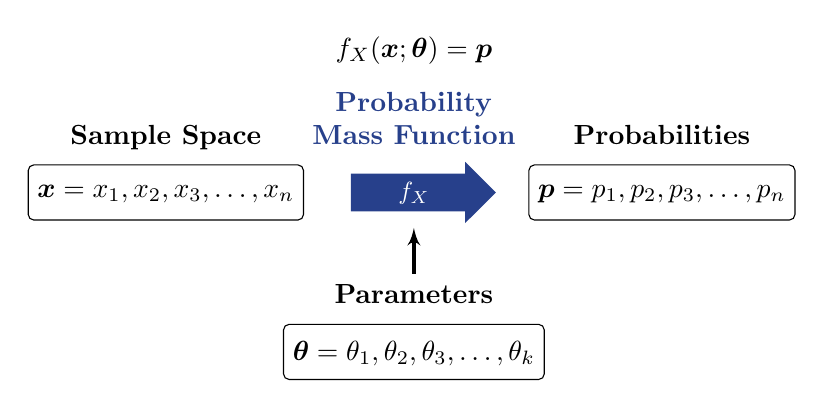
\begin{tikzpicture}[>=stealth,scale=0.9]
\definecolor{royalblue2}{RGB}{39,64,139};
\node [rectangle,
       draw,
       rounded corners= 2pt,
       text depth=0.25ex,
       minimum height = 7mm](ss) at (0,0) {$\boldsymbol{x}=x_1,x_2,x_3,\ldots,x_n$};
\node [rectangle,
       draw,
       rounded corners= 2pt,
       text depth=0.25ex,
       minimum height = 7mm](ps) at (7,0) {$\boldsymbol{p}=p_1,p_2,p_3,\ldots,p_n$};
\node [single arrow,
       fill=royalblue2,
       single arrow head extend=1.1ex,
       transform shape,
       minimum height=0.9cm,
       text depth=0.25ex, text=white] (fx) at (3.5,0) {$\quad\;\; f_X\quad\;\;$};
\node [text depth=2.25ex,
       text height= 5ex,
       anchor=south,
       yshift=-3.5ex](sst) at (0,0.75) {\textbf{Sample Space}};
\node [text depth=2.25ex,
       text height= 5ex,
       anchor=south,
       yshift=-3.5ex](pst) at (7,0.75) {\textbf{Probabilities}};
\node [shape=rectangle,
       text depth=2.25ex,
       color=royalblue2,
       align=center,
       text height= 5ex,
       anchor=south,
       yshift=-3.5ex](pmf) at (3.5,0.75) {\textbf{Probability}\\
	\textbf{Mass Function}};
\node [text depth=2.25ex,
       text height= 5ex,
       anchor=south,
       yshift=-3.5ex] (pt) at (3.5,-1.5) {\textbf{Parameters}};
\node [rectangle,
       draw,
       rounded corners = 2pt,
       text depth=0.25ex,
       minimum height = 7mm] (pts) at (3.5,-2.25) {$\boldsymbol{\theta}=\theta_1,\theta_2,\theta_3,\ldots,\theta_k$};
%\node [align=center,
%       shape=rectangle,
%       rounded corners = 3pt,
%       draw](formula) at (3.5,4) {\textbf{\Large{Scary~Math!}}\\
%	$f_X\!\left(\boldsymbol{x};\boldsymbol{\theta}\right)=\boldsymbol{p}$};
%\draw [rounded corners=5pt] (-2.5,-3) rectangle (9.5,2.65);
\node at (3.5,2) {$f_X\!\left(\boldsymbol{x};\boldsymbol{\theta}\right)=\boldsymbol{p}$};
\draw[->,>=latex', very thick] (3.5,-1.15) to (3.5,-0.5);
\end{tikzpicture}
\end{document}
